\mysubsection{Message et communication asynchrone}

\ifbook{
  \mysubsubsection{Problématique de la communication asynchrone}
    \paragraph{} Depuis les débuts de l'informatique, le besoin d'une communication \textbf{asynchrone} entre
    deux processus ou deux programmes est présent et les problématiques liées à ce genre de communication sont
    bien connues. Tout langage de programmation fournit les primitives nécessaires à l'implémentation d'une telle
    communication, mais on fait désormais plus souvent appel à des \textit{middlewares} dédié. Ainsi, le
    monde du \textit{Message Oriented Middleware} a émergé, autant pour faciliter le développement qu'assurer une
    bonne gestion des messages échangés.
}

\ifslide{
  \begin{frame}{Problématique de la communication asynchrone (1/2)}
    \begin{block}{Motivations}
      \begin{itemize}
        \item \textit{fire and forget}
        \item \textit{can't wait}
        \item \textit{producteur / consommateur}
      \end{itemize}
    \end{block}
  \end{frame}
}

\ifbook{
 \paragraph{} Avant d'avancer plus en avant dans la description du fonctionnement générale de ces
 \textit{middlewares} étudions rapidement les cas d'utilisation qui motivent leurs utilisations.
 Sans être exhaustive, voici quelques exemples, volontairement très générique, de cas d'utilisation
 où l'on souhaite généralement mettre en place une communication \textbf{asynchrone} entre deux
 processus:

 \begin{description}
   \item [\textit{"fire and forget"}] Un processus souhaite communiquer une information à un autre,
   sans attendre que ce dernier est fini son traitement pour continuer (ex: journalisation des
   opérations d'une application). Généralement, dans ce genre de cas, le traitement qui doit être
   réalisé par le second processus n'a pas d'impact sur celui réalisé par le premier, qui peut donc
   continuer sans attendre.
   \item [producteur et consommateur] Problème d'algorithmique classique, le
   \mylink{http://fr.wikipedia.org/wiki/Mod\%C3\%A8le\_producteur-consommateur}{modèle
   producteur/consommateur} est un cas d'étude classique d'une communication asynchrone. En
   quelques mots, le processus producteur dépose, dès qu'il peut, une demande de traitement dans une
   sorte de "boite à message", qu'un processus consommateur, quand il le souhaitera ou pourra,
   récupérer, et effectuer le traitement nécessaire.
 \end{description}
}


\ifslide{

  \begin{frame}{Problématique de la communication asynchrone (2/2)}
    \begin{block}{Problématiques}
      \begin{itemize}
        \item gestion d'erreur
        \item gérer les queues
        \item persistance (ou non) des messages
      \end{itemize}
    \end{block}
  \end{frame}
}

\ifbook{

  \paragraph{} La nature même de la communication induit rapidement le besoin de gérer l'état des
  messages échangés. En effet, à partir du moment où la réception d'un message n'est pas immédiate,
  il va souvent devenir nécessaire de s'assurer que ces derniers soit persistés et administrer. Il
  s'agit d'un point est un important, car si les messages ne sont jamais consommés par exemple, le
  système peut rapidement se retrouver dans un état instable, car débordé de message qui ne
  "disparaissent jamais"...

  \paragraph{} Il devient rapidement nécessaire de gérer donc des files d'attentes (\textit{Queues} en
  anglais) ainsi que des erreurs de transmission. Au regard de ces quelques points, il apparait
  clairement que tout ceci offre là encore, un terrain d'investigation intéressant pour la conception
  de \textit{middleware}...
}

\ifslide{

  \begin{frame}{Message Oriented Middleware (MOM)}
    \begin{block}{Domaines}
      \begin{itemize}
        \item Publish/Subscribe (pub/sub) : n producteurs, n consommateurs
        \item Point To Point (PTP) : n producteurs, 1 consommateur
      \end{itemize}
    \end{block}

    \begin{center}
      \includegraphics[scale=0.3]{img/topic-queue.png}
    \end{center}
  \end{frame}
}

\ifbook{

 \paragraph{} Un autre avantage des \textit{MOM} (\textit{Message Oriented Middleware}) est aussi la
 capacité d'effectuer une communication de 1 à n tiers aisément. En effet, une fois un message remis
 à tel programme, ce dernier peut le mettre à disposition d'un ou plusieurs processus. Ainsi, on
 peut disposer de plusieurs processus (ou même machine) prête à consommer les messages transmis.

 \mysubsubsection{Un exemple de standardisation des MOM : Java Message Service}

 \paragraph{} Sans rentrer dans les détails de cette API Java\footnote{Voir
 \mylink{http://en.wikipedia.org/wiki/Java_Message_Service}{Java Message Service}}, nous
 pouvons juste retenir que, reprenant la théorie évoqué plus haut, cette spécification définit
 l'API que doit supporter et respecter un MOM implémenté en Java.

 \paragraph{} En plus de fournir les services d'administration et de diffusion évoqués, cette
 API assure aussi un fort \textbf{découplage} entre le logiciel client (utilisant l'API) et
 l'implémentation de la spécification JMS qu'il utilise. Ceci permet ainsi de facilement remplacer
 une implémentation par une autre - sans altérer le comportement du programme\footnote{Bien
 évidemment, les performances, comme les limites du composant varieront selon l'implémentation
 utilisée - toute la difficulté étant donc le choix judicieux de cette dernière.}.

 \paragraph{} La figure \ref{jms-steps} présente, dans les grandes lignes, les composants logiciels
 impliqués lors d'une communication aynchrone utilisant JMS.

  \begin{center}
    \begin{figure}
      \includegraphics[scale=0.3]{img/jms-steps.png}
      \label{jms-steps}
      \caption{Vue générale d'une communication asynchrone à l'aide de JMS}
    \end{figure}
  \end{center}
}

\ifslide{

   \begin{frame}
     \begin{block}{Invocation JMS}
       \begin{itemize}
         \item Localiser le driver JMS lookup JNDI. Le driver est une connection
 factory
         \item Créer une connection JMS obtenir une connection à partir de la
 connection factory
         \item Créer une session JMS :Il s'agit d'un objet qui va servir à recevoir et
 envoyer des messages. On l'obtient à partir de la connection.
         \item Localiser la destination JMS: Il s'agit du canal sur lequel les
 messages sont emis ou recus. Normalement, c'est réglé par le
 déployeur. On obtient la destination via JNDI.
         \item Créer un producteur ou un consommateur JMS. Utilisés pour écrire
 ou lire un message. On les obtient à partir de la destination et de la
 session.
         \item Envoyer ou recevoir un message
       \end{itemize}
     \end{block}
   \end{frame}

   \begin{frame}{Message Oriented Middleware (MOM)}
     \begin{center}
       \includegraphics[scale=0.3]{img/jms-steps.png}
     \end{center}
   \end{frame}
 }

\ifbook{

  \mysubsubsection{Autre considérations relatives à l'usage des MOM}

  \paragraph{} Bien qu'en première anlayse les MOMs soient des outils relativements simple dans leur
  concept (une simple pile de message), leurs usages entrainent vite l'apparition de problématiques,
  déjà évoqués précédemment, telles que:
  \begin{description}
    \item[transactionnalité] Le MOM peut rapidement se trouver parti prenant d'échange
    transactionnel et devra donc être en mesure de supporter les contraintes qu'impliquent un tel
    contexte - spécialement si ce dernier doit prendre part à des transaction distribués (voir le
    \textit{Two Phase Commit} étudié précédemment).
    \item[sécurité] De la même manière, tous les problématiques usuels de sécurité, ainsi que les
    méchanismes classiques associés, se retrouvent lors du dépoiement d'un MOM au sein d'un
    système. Un MOM offre donc généralement des fonctionnalités d'authentification et
    d'authorisation et peut utiliser différents mécanismes (certificat, mot de passe, ...) pour les
    implémenter.
  \end{description}

}

\ifslide{

  \begin{frame}{Message Oriented Middleware (MOM)}
    \begin{block}{Domaines}
      \begin{itemize}
        \item Transactions and MBD %: La production et la consommation du message sont dans deux transactions séparées...
        \item Sécurité %: Les MDB ne reçoivent pas les informations de sécurité du producteur avec le message.
      \end{itemize}
    \end{block}
  \end{frame}
}

\ifbook{

  \mysubsubsection{Rôle d'un MOM dans l'architecture d'un système}


  \paragraph{} Disposer d'un MOM au sein de son architecture logicielle apporte de nombreux
  avantages. Premièrement, on dispose d'un mécanisme permettant d'établir, de manière indépendante
  du protocole sous jacent, une \textbf{communication par message}, dans laquel le MOM fait office
  d'intermédiaire.

  \paragraph{} Ce rôle d'intermédiaire permet au MOM d'apporter plusieurs fonctionnalités
  très intéressantes en termes de \textbf{découplage} et de stratégie de \textit{montée} ou
  \textbf{répartition} de charge. Ainsi, on peut en effet imaginer, par exemple, utiliser un MOM
  pour faire office de tampon temporaire entre deux systèmes, pour adapter une différence de
  fréquence entre le système producteur de message, très rapide, et celui ou ceux qui les consomment
  et traitent, vraisemblablement plus lent.

  \paragraph{} Un autre exemple est le \textbf{routage de message}. Une application se contente d'envoyer des
  messages à un MOM, et celui ci redistribue les messages, selon leur métadonnées, à différents
  systèmes consommateurs. Bien évidemment, on peut aussi placer plusieurs instances du MOM en parallèle et
  effectuer, entre ces différentes instances, un équilibrage de charge.

  \paragraph{} Tout ces exemples soulignent bien la souplesse et la flexibilité qu'un MOM peut
  donner à une architecture logicielle. Ces derniers accroissent nettement la complexité d'un
  système.
}

\ifslide{
  \begin{frame}
    \begin{block}{Advantages}
      \begin{itemize}
        \item message-based communications protocol
        \item store/buffer
        \item routing / load balancing
      \end{itemize}
    \end{block}
  \end{frame}

  \begin{frame}{Standardisation ?}
    \begin{block}{No Standard yet :( (API only) }
      \begin{itemize}
        \item JMS (Java Messaging System)
        \item MSMQ (Microsoft Message Queuing)
        \item Amazon Simple Queue Service
      \end{itemize}
    \end{block}

    \begin{block}{Protocol}
      \begin{itemize}
        \item AMQP (Advanced Message Queuing Protocol) - protocole
        \item STOMP (Streaming Text Oriented Messaging Protocol)
      \end{itemize}
    \end{block}
 \end{frame}

 %\demoframe{Communication Asynchrone}{ Exemple avec JMS}
}

\mysubsection{Gestion des processus métiers (BRMS)}

\ifbook{
  \paragraph{} Une des problématiques les plus récurrentes dans les projets informatiques est la
  difficulté, pour les développeurs, de comprendre les besoins fonctionnels associées à
  l'application qu'ils développent. Un lourd travail de spécification est généralement réalisé pour
  permettre aux développeurs de bien comprendre les différents aspects, très proche du métier des
  utilisateurs du logiciel.

  \paragraph{} En outre, la nature changeante de la plupart des professions fait qu'il est rapidement
  nécessaire de modifier une partie de la logique fonctionnelle de l'application. Là encore, un
  difficile travail de transfert est à effectuer entre les personnes disposant des réels connaissances
  métiers et les développeurs.

  \paragraph{} On notera d'ailleurs que cette problématique explique, pour beaucoup, le succès de
  feuilles de calculs (qu'il s'agisse de \mylink{}{Excel} ou \mylink{}{Libre Office Calc}). En fait,
  ces dernières permettent à des comptables ou des fiscalistes, par exemple, de facilement concevoir
  une sorte de "petit programme" faisant exactement ce dont ils ont besoin, sans passer par
  l'intermédiaire d'un dévelopeur. On trouve d'ailleurs de nombreux expert de ce genre d'outil dans
  les salles de marché, où il est souvent nécessaire de concevoir un logiciel de calcul relativement
  avancé en quelques minutes seulement...

  \paragraph{} Le constat que venons d'effectuer à amené une nouvelle technologie, les
  \textbf{moteurs de règle} à émerger - ou en anglais \textit{Business rule management system}. L'idée
  sous jacente de cette nouvelle technologie est, comme souvent, assez simple: fournir un outil
  générique conçu pour implémenter et concevoir des règles dites "métiers". Les règles définies à
  l'aide de cet outil s'intègreront ensuite dans une application.

  \paragraph{} Ainsi, des experts fonctionnels, avec peu ou pas de compétence de programmation,
  pourront être en charge de l'implémentation des règles métiers que les développeurs pourront
  intégrer dans leur propre travail. Les avantages de cette approche sont
  flagrants:

  \begin{itemize}
    \item diminuer le besoin de développement supplémentaire pour modifier les fonctionnalités
    purement métier d'une application ;
    \item donner plus de contrôle sur la logique de décision et la gestion du processus métier en
    général à des experts fonctionnels plutôt qu'à des développeurs.
  \end{itemize}

  \paragraph{} Le domaine étant encore finalement assez récent, on ne trouve pas encore
  \textbf{standard} - bien que des initiatives dans ce sens avance rapidement\footnote{Comme par
  exemple la standardisation d'une API Java avec la JSR-94}, et il existe donc
  encore de grande différences entre les produits \textit{middleware} disponibles sur le marché. On
  peut néamoins retenir que tout \textbf{moteur de règles} est constitué des éléments suivants:

  \begin{description}
      \item[dépôt] ce dernier permet d'externaliser le code "métier" du reste de
      l'application
      \item[outils] permet à la fois aux développeurs et aux spécialistes métiers de travailler
      ensemble.
      \item[conteneur d'exécution\footnote{Oui, encore un nouveau conteneur d'exécution...}] pour
      exécuter les règles définies pour l'application et interagir avec elle.
  \end{description}

  \paragraph{} Un exemple relativement complet, et ouvert, de ce type de \textit{middleware} est sans
  conteste \mylink{https://community.jboss.org/wiki/JBossRules}{JBoss Rules}, anciennement appelé
  Drools. Pour plus d'information précise sur ce type de produit, le lecteur pourra donc se référer
  à la documentation JBossRules disponible en ligne, ainsi qu'à la communauté associée.
}

\ifslide{

\begin{frame}
  \begin{block}{Disclaimer}
    \begin{center}
      \Large{I suck}
    \end{center}
  \end{block}
\end{frame}


\begin{frame}{Business Process Management}
  \begin{block}{Motivations}
    \begin{itemize}
      \item developer/business expert
      \item lifecycle
    \end{itemize}
  \end{block}
\end{frame}


\begin{frame}
  \begin{block}{What makes a BRM ?}
    \begin{itemize}
      \item \textbf{Repository} %, allowing decision logic to be externalized from core application code
      \item \textbf{Tools} % allowing both technical developers and business experts to define and manage decision logic
      \item \textbf{Runtime environment} %, allowing applications to invoke decision logic managed within the BRMS and execute it using a business rules engine
     \end{itemize}
  \end{block}
\end{frame}


%The top benefits of a BRMS include:[2]
\begin{frame}
  \begin{block}{What's the point ?}
    \begin{itemize}
      \item Reduced or removed reliance on IT departments for changes in live systems
      \item Increased control over implemented decision logic for compliance and better business management
      \item The ability to express decision logic with increased precision %, using a business vocabulary syntax and graphical rule representations (decision tables, trees, scorecards and flows)
      \item Improved efficiency of processes through increased decision automation
      \item Most BRMS vendors have evolved from rule engine vendors to provide business-usable software development lifecycle solutions, based on declarative definitions.
    \end{itemize}
  \end{block}
\end{frame}

\begin{frame}
  \begin{block}{Standardisation}
    \begin{itemize}
      \item No standard for business rules defined within a BRMS
      \item a standard for a Java Runtime API for rule engines JSR-94.
    \end{itemize}
  \end{block}

  \begin{block}{Other standards (under development)}
    \begin{itemize}
      \item OMG Business Motivation Model (BMM): A model of how strategies, processes, rules, etc fit together for business modeling
      \item OMG SBVR: Targets business constraints as opposed to automating business behavior
      \item OMG Production Rule Representation (PRR): Represents rules for production rule systems that make up most BRMS' execution targets
      \item W3C RIF: A family of related rule languages for rule interchange
      \item Many standards, such as domain-specific languages, define their own representation of rules, requiring translations to generic rule engines or their own custom engines.
    \end{itemize}
  \end{block}
\end{frame}
}


\ifslide{
  \mysubsection{Sécurité}
  \begin{frame}{Qu'est ce que la sécurité applicatives ?}
  \begin{block}{Motivations}
    \begin{itemize}
      \item aspect généralement technique
      \item protection des ressources en fonction de l’utilisateur qui y accede
      \item \textbf{autorisation} d’acces pour un \textbf{utilisateur} à une \textbf{ressource}
    \end{itemize}
  \end{block}

  \begin{block}{Procédure}
    \begin{itemize}
      \item Identification
      \item Autorisation
    \end{itemize}
  \end{block}
\end{frame}

\begin{frame}
  \begin{block}{Implémentation}
    \begin{itemize}
      \item HTTP Basic
      \item Certificat X509
      \item ...
    \end{itemize}
  \end{block}
\end{frame}

}

\mysubsection{Modèle de programmation}
% EJB
\ifbook{
    \mysubsubsection{Propos de cette section}

    \paragraph{} Comme l'a explicité, dans les premiers chapitres, la description des nombreux
    "conteneurs d'exécutions" dans lesquelles les applications modernes sont déployées. Un grand
    nombre de mécanismes, associés aussi à des certaines contraintes de programmation donne un
    cadre puissant et robuste à l'application.

    \paragraph{} Malgré tout ceci, la réalisation d'application reste un sujet vaste, et il
    est fréquent que, dans le cadre d'un projet, on décide d'utilise un ou plusieurs autres
    \textit{frameworks} supplémentaires, fournissant généralement un cadre de développement estimé
    encore plus efficase ou approprié pour l'implémentation désirée.

    \paragraph{} Rien que dans le monde Java, on distingue une kyrielle vertigineuse de ces
    \textit{frameworks} parmi lesquelles on citera juste les suivants, à titre d'exemple:

    \begin{itemize}
      \item \mylink{http://www.springsource.org/}{Spring}: un \textit{framework} très souvent
      utilisé et conçu pour offrir un cadre robuste, simple et complet aux développement
      d'applications \textit{web} modernes. Il est souvent présenté comme une alternative plus
      simple à l'utilisation des standards associés à JEE.
      \item \mylink{http://struts.apache.org/}{Struts}: un très célèbre \textit{framework} adaptant
      le classique modèle
      \mylink{http://fr.wikipedia.org/wiki/Mod\%C3\%A8le-Vue-Contr\%C3\%B4leur}{MVC} à la
      réalisation d'application \textit{web}.
      \item \mylink{http://www.oracle.com/technetwork/java/javaee/javaserverfaces-139869.html}{JSF}
      et ses implémentations: standard issu du monde JEE, JSF propose un modèle de programmation
      dédié à la réalisation d'application \textit{web} métiers. Un des objectifs avoués du standard
      et de ses implémentations est de permettre un développement similaire à celui d'application
      dites "lourdes", en prenant en charge, autant que possible, les spécificités des technologies
      internet.
      \item ...
   \end{itemize}

   \paragraph{} Fort de ce simple constat, il apparait évident que dresser un tabelau exhaustif,
   même limiter à l'univers Java/JEE Open Source et standard, formerait une excellente treizième
   tâche pour Hercule, et dépasserait totaltement le cadre de cet exposé.

   \paragraph{} Néanmoins, ce genre de composant formant une partie intégrante du paysage associé
   aux \textit{middleware}, il est pertinent, dans le cadre de ce cours, de présenter l'un d'eux. Cette
   analyse donnera, espérons-le, au lecteur, une grille de lecteur suffisante pour entreprendre lui
   même ce travail de "décorticage" technologique lorsqu'il sera confronté à la toute dernière
   déclinaison "à la mode" de ces \textit{frameworks}.

   \paragraph{} Cette section présente donc, de manière volontairement très sommaire, les grandes
   lignes du modèle de programmation promût par le standard EJB, dans sa troisième version (de loin
   à ce jour la plus simple et réussie). L'objectif de ce standard, et de ses implémentations, est
   donc - comme nous allons le voir, la normalisation de la définition et de l'utilisation de
   \textbf{composant distribué}.

   \paragraph{} \textit{Le lecteur prendra soin de noter immédiatement l'importance de bien saisir
   quel est l'objectif que cherche à atteindre le framework et quel modèle de programmation
   il promeut. En effet, il est, de manière très regrettable, fréquent de
   voir des projets embarqués une kyrielle de composants, plus ou moins standard, plus ou moins
   ouvert, plus ou moins robustes, mais surtout plus ou moins utile à l'application. Cette
   empilement technologique confus, au delà de rendre le code de l'application très complexe, a
   aussi l'effet de bord d'augmenter grandement la difficulté de sa mise en oeuvre.}

   \mysubsubsection{Motivations et objectifs des EJB}

   \paragraph{} L'objectifs du standard EJB est de définir un ensemble d'API pour faciliter et
   normaliser la conception de composant \textbf{distribué}, et de permettre ainsi de construire
   des applications où les traitements sont réalisés sur différentes machines, au sein de différents
   serveurs d'application.

   \paragraph{} L'enthousiasme certain que le modèle a suscité lors de sa première parution a
   abouti une forte adoption - spécialement dans le cadre de la conception d'application
   \textit{web}. On notera au passage que ces dernières ne nécessitent aucunement la mise en place
   d'un modèle distribué, et que l'abus d'utilisation des EJB dans ce contexte est aussi un bon
   contre exemple à retenir.

   \begin{center}
     \includegraphics[scale=0.3]{img/ejb-overview.png}
   \end{center}

   \paragraph{} La spécification définit la notion de \textit{bean} - à traduire ici comme
   "conteneur"\footnote{Hé oui, encore un conteneur !}. EJB étant une norme spécifique à Java et à
   la spécification \mylink{TODO}{JEE}, la    notion de \textbf{bean} s'applique en effet à un
   objet\footnote{Pour rappel, un objet est une instanciation en mémoire d'un classe} implémentant une
   fonctionnalité ou un service (technique ou métier) au sein de l'application.

   \paragraph{} En plus de définir un ensemble de caractéristiques spécifiques des \textit{beans},
   la spécification permet de rendre le composant \textbf{local} - c'est à dire s'exécutant au sein
   du même serveur d'application que son client, ou distant de manière complètement transparente.
   Ceci permet donc de séparer, sur des serveurs distincts, des composants ou des traitements
   métiers.

   \paragraph{} En définissant la manière dont ces composants distribués sont utilisées par les
   applications, la spécification permet aussi de décharger ces dernières d'un ensemble de tâches
   techniques (la gestion du cycle de vie du composant ou la sécurisation des échanges par exemple)
   et d'en rendre le serveur d'application responsable. Le respect du standard permettant, en outre,
   de aisément migrer l'application d'un fournisseur de serveur d'application à un autre...\footnote{
   ...Tout du moins en théorie. Il n'est pas si aisé que ça d'effectuer la migration d'une application
   EJB d'un serveur d'application à une autre, mais l'effort nécessaire n'est en rien comparable à ce que
   fût les problèmes de portabilités entre systèmes d'exploitation. À titre d'exemple,
   certaines entreprises ont réussi à migrer d'un serveur JEE à un autre en quelques semaines à peine.}
}

\ifslide{
  \begin{frame}{Exemple de modèle de programmation: EJB}
    \begin{center}
      \includegraphics[scale=0.3]{img/ejb-overview.png}
    \end{center}
  \end{frame}

  \begin{frame}
    \begin{block}{Motivations}
      \begin{itemize}
        \item EJB définit des contrats associés à un Bean
        \item Déploiement local ou distant
      \end{itemize}
    \end{block}
  \end{frame}
}

\ifbook{
  \mysubsubsection{Quelques exemples d'EJB}

  \paragraph{} Sans rentrer dans les détails les plus techniques, cette partie va présenter
  quelques caractéristiques que les fameux \textbf{beans} de la spécification EJB peuvent avoir.
  L'analyse de ces quelques caractéristiques devraient en effet éclairer le lecteur sur l'intérêt de
  l'utilisation de cette technologie dans le cadre d'une application, et, par effet de bord,
  l'intérêt de l'utilisation des \textit{frameworks} en général.

  \paragraph{} La norme EJB étant extrêmement vaste et riche, notre présentation se limitera à une
  brève description de certains de ses composants. Nous allons donc étudier les trois types de
  \textbf{beans} suivants:

  \begin{itemize}
    \item \textit{Stateful Bean} et \textit{Stateless Bean}
    \item \textit{Entity Bean}
    \item \textit{Message-Driven Bean}
  \end{itemize}

  \mysubsubsection{Exemple de composant sans ou avec état}

  \paragraph{} Comme décrit plus haut, un composant, au sens EJB, fournit à ses utilisateurs un
  service technique ou métier. Il implémente, pour le compte de l'application, une fonctionnalité
  par exemple. Selon ce traitement, le composant a besoin ou non de conserver un \textbf{état} entre
  chaque requête.

  \paragraph{} Prenons un exemple simple et concret en imaginant un composant dont la charge est de
  vérifier que le mot de passe d'un utilisateur est valide. Selon la manière dont ce mécanisme est
  implémenté, ce composant peut ou non avoir un \textbf{état}.

  \paragraph{} Première implémentation, le composant reçoit une requête avec le nom d'utilisateur et
  le mot de   passe. Il se connecte à un annuaire d'entreprise, probablement par le bais du
  protocole LDAP, vérifie si le mot de passe est correct, ferme la connection et retourne le
  résultat à son composant client.

  \paragraph{} Dans cette première implémentation, le composant est \textbf{sans état} - ou
  \textit{stateless}. En effet, il n'a besoin de ne conserver aucune information entre les requêtes
  qu'il reçoit. Cette même instance peut être utiliser pour une nouvelle requête sans aucun effet de
  bord. En essence, à la fin de la requête, le composant est rigouresement dans le même état
  qu'avant la requête.

  \paragraph{} Modifions maintenant cette implémentation pour lui ajouter un système de cache. En
  effet, comme la communication vers l'annuaire est coûteuse - il s'agit d'un appel réseau après
  tout, il semble pertinent de placer toute information récupérée dans un cache local au composant. À
  chaque requête, le composant vérifiera d'abord si il ne dispose pas de l'information recherchée,
  et sinon, se connectera à l'annuaire. Dans le cas où il disposera déjà de l'information en
  question, le traitement de la requête sera bien évidement beaucoup plus rapide.

  \paragraph{} Cette nouvelle version du composant vient d'introduire un \textbf{état}. Désormais, à
  l'issue d'une requête, il n'est pas garanti que le composant retrouve son état initiale - il peut
  en effet voir son cache augmenté d'une entrée. Le composant est désormais \textit{stateful} et cet
  aspect va grandement modifier la manière dont le serveur applicatif va gérer son cycle de vie.

  \mysubsubsection{Les entités}

  \paragraph{} À la parution de la spécification JEE, ces composants désignés sous le nom de
  \textit{entity beans} ont beaucoup séduit les développeurs et les architectes logicielles. En
  effet, ils portaient avec la eux la promesse de simplifier grandement la gestion d'un aspect
  complexe des applications: la \textbf{persistence}. Si les premières montures de la spécification
  (EJB 1.x et 2.x) sont loin d'avoir tenu ces promesses, la plus récente version (EJB 3.x)
  utilisant le standard JPA facilite réellement la gestion de cette problématique.

  \paragraph{} En effet, un \textbf{entity bean} est un objet conçu pour représenter un ensemble de
  donnée métier. Par exemple, un utilisateur du logiciel (nom, prénom, nom d'utilisateur) ou un
  objet du catalogue, dans le cas d'un site de e-commerce. Cet objet ne contient généralement que
  peu de logique, il se contente de regrouper l'ensemble des attributs de l'entité qu'il représente.

  \paragraph{} Clarifions tout d'abord ce que l'on entend par \textbf{persistance}. Une applications
  Java n'est, au final, qu'un ensemble d'objets instanciés en mémoire. Une partie de ces objets
  représentent souvent des données métiers (les données d'utilisateurs, les produits placés dans le
  panier d'un utilisateur, etc..). Ces informations devant souvent survivre bien au délà de leur
  utilisations par l'application, il est donc nécessaire de le sauvegarder sous une forme durable -
  et non seulement en mémoire.

  \paragraph{} Les bases de données relationnelles, utilisant le langage de requête SQL, sont depuis
  longtemps, à tort ou à raison, devenu l'outil de référence pour confier la persistance des données
  d'une application. Néanmoins, leur modèle de représentation des données - un ensemble de tables
  liées entre elles par des contraintes d'intégrités et des relations, est fondamentalement assez
  différent d'un modèle objets, ou des instances hérites les unes des autres et s'aggrègent.

  \paragraph{} Cette différence profonde est en fait un simple problème \textbf{d'impédance} entre
  la représentation en mémoire des objets et la vision relationnelle des bases de données. Pour
  résoudre ce problème, l'industrie - par le truchement du \textit{framework Open Source}
  \mylink{ToDO}{Hibernate} ou du produit \mylink{}{TopLink}, a souvent eu recours à une approche
  désignée sous le nom de \textit{Object - Relation Mapping (ORM)}.

  \paragraph{} Cette approche est en fait assez simple, elle consiste à fournir à un outil la
  description du travail de transformation à effectuer à partir des objets ou des données issues de
  la base données pour les adapters à la transformation cible. Cet outil allège donc grandement le
  travail des développeurs, pour qui, par exemple, se contente d'invoquer une méthode "sauvegarder"
  pour mettre à jour, en base, un objet qu'ils manipulent.

  \paragraph{} Les outils d'\textit{ORM} prendront en effet à leur charge la gestion de la complexité
  sous jacente du= modèle de données (comme la mise à jour de plusieurs tables si les données de l'objet
  sont sauvegardés sur plusieurs d'entre elles). En outre, effet de bord assez appréciable,
  l'\textit{ORM} fournit une excellente abstraction de la base de données utilisée - abstraction
  standardisée par JPA qui plus est, et permet d'envisager de changer de fournisseur de base de
  données aisément.\footnote{Comme précédemment, on notera que ce genre de migration n'est pas si
  aisée et pose parfois des problèmes, entres autres, de performance. Néanmoins, elles restent tout à
  fait envisageable, dans des délais raisonnables - pour peu que l'application réalisée respecte le
  standard.}

  \paragraph{} Dans le cadre des \textbf{Entity Beans} de EJB 3.x, c'est donc JPA qui est retenu
  pour assurer la persistence des \textbf{Entity Beans}. Comme ces derniers voient leur cycle de vie
  confiés au serveur JEE, le travail des développeurs est encore plus allégé, car ils n'ont même
  plus à déclarer de manière explicite que l'objet doit être mise à jour en base de données - le
  conteneur étant, la plupart du temps, capable de le détecter par lui même !

  \mysubsubsection{Message Driven Bean}

  \paragraph{} Dernier composant issu de la spécification EJB que nous évoquerons dans cette section
  les \textit{Message Driven Bean} (MDB) sont, comme leurs nom anglais l'indique, des composants
  invoqués par le serveur JEE à la réception d'un message transmis par un MOM. L'avantage de ces
  compposants, en plus d'être créer et gérer par le serveur, est qu'ils libèrent le développeur de
  tout la gestion propre à l'utilisation d'un MOM.

}

\ifslide{

  \begin{frame}
    \begin{block}{Standard}
       \begin{itemize}
         \item Portabilité des beans sur différents serveurs EJB
         \item Indépendance du fournisseur
      \end{itemize}
    \end{block}
  \end{frame}

  \begin{frame}
    \begin{block}{Types}
      \begin{itemize}
        \item Session Bean
        \item Entity Bean
        \item Message-Driven Bean
      \end{itemize}
    \end{block}

    \begin{center}
      Si l'on utilise un Session Bean quel impact sur l'architecture de l'application ?
    \end{center}

  \end{frame}
}

\ifbook{
  \mysubsubsection{Synthèse}

  \paragraph{} Sans aller plus loin dans la description des apports de la spécification EJB, dans le
  cadre de développement d'applications JEE, nous pouvons déjà faire une synthèse pédagogique qui
  devrait éclairer le lecteur sur l'intérêt de l'utilisation d'un \textit{framework} et du modèle de
  programmation qu'il promeût.

  \paragraph{} En effet, à la lecture de la description des différents composants évoqués, il
  apparait clairement élégant et avantageux, de les utiliser, si approprié dans le cadre d'un
  développement, pour réduire la quantité de code à produire, et aussi simplifier et standardisé le
  développement. En outre, et c'est là un point crucial, en utilisant un tel \textbf{canevas}, on
  s'assure que les développeurs suivront un modèle de programmation sain et reconnu.

  \paragraph{} Pour illustrer ce point, suppossons qu'une application, réalisée par un développeur
  brillant utilise les éléments suivants:

  \begin{itemize}
    \item un ensemble de service, avec ou sans état, mais ne suivant pas le standard EJB
    \item certains traitements sont déclenché lors de la réception de message provenant d'un MOM, mais
    l'implémentation ne suit pas la norme des MDB.
    \item la persistance est réalisée de manière spécifique, utilisant simplement des requêtes SQL,
    directement executées sur la base de données.
  \end{itemize}

  \paragraph{} Une telle application, en plus de problème de poser potentiellement des problèmes de
  configuration et d'adhérence à la base de données utilisée, posent aussi un problème encore plus
  pragmatique : le recrutement de développeurs pour travailler dessus. Seul un développeur brillant et
  maitrisant les différentes techniques utilisées par le concepteur original sera en mesure
  d'assurer la maintenance du code et l'ajout de nouvelles fonctionnalités.

  \paragraph{} À l'inverse une application JEE standard pourra non seulement être maintenue par la
  plupart des développeurs de l'industrie, pour peu qu'il soit famillié avec le standard, et pourra
  être optimisée lors de son déploiement, à l'aide des nombres aspects de son fonctionnement qui ont
  été déportés vers le serveur JEE.

  \paragraph{} Cette conclusion n'est évidement par propre au standard EJB. Elle s'applique à
  l'utilisation du célèbre \textit{framework} \mylink{TODO}{Spring} ou encore dans le monde Ruby, de
  \mylink{TODO}{Ruby On Rails}. Ce qui est essentiel de retenir c'est qu'un modèle de programmation
  - apporté par un \textit{framework}, permet d'accéler et de faciliter grandement le développement
  d'application.

  \paragraph{} Néanmoins, il faut aussi retenir que leur utilisation est très \textbf{structurante}
  et que si ils ne sont pas donc pas adaptés au besoin de l'application, ils peuvent devenir une
  entrâve, en empêchant littéralement le développeur de réaliser les fonctionnalités demandées.
}


\mysection{C - Application distribuée et intégration (11/01/2012)}

\abstractframe{Élargissant le spectre au-delà du périmètre de l'application,
cette partie étudie les services et composants proposés par les
\textit{middlewares} pour dialoguer et s'intégrer à son environnement et plus
spécialement à la nature \textbf{distribuée} du système d'information dans lequel
elle évolue.}{../img/overview-integration.png}

\mysubsection{Sources de données} %{\includegraphics[scale=1]{../img/pool2.jpg}}

\ifbook{
  \mysubsubsection{Qu'est ce qu'une ressource ?}

\paragraph{} Dans le domaine du \textit{middleware}, on utilise régulièrement des abstractions, du
plus au niveaux possibles, pour créer des composants les plus génériques possibles, pouvant donc
être ainsi réutilisé autant que possible. En outre, ces composants peuvent être configurés pour
répondre à des problématiques similaires. Une de ces abstractions les plus courament utilisée est la
notion de \textbf{ressource}\footnote{Là encore, l'expérience très orientée Java/JEE de l'auteur de
ce document influence peut être la sémantique. Fort heureusement, les concepts décrits ici devraient
pouvoir s'appliquer à toutes autres technologies.}.

\paragraph{} Une ressource désigne en fait une application tierse, un service au sens le
plus générique du terme, que l'application accède pour transmettre et recevoir des donnnées. Une
ressource peut donc être un simple fichier ou quelquechose d'aussi complexe qu'une base de données
relationnelle.

\paragraph{} Les entités désignées par ce terme sont volontairement très abstraite pour permettre d'
utiliser élements ou mécanismes de nature très différentes d'une manière identique. Mais, aussi
abstrait soient elles, les ressources partagent tout de même certains point en communs:

\begin{description}
  \item[processus externe] une \textbf{ressource} est forcément externe au
  processus de l'appication. Un cache local, par exemple, même s'exécutant dans un processus séparé,
  ne peut pas réellement être considéré comme \textbf{ressource}. Si le cache est dans une
  application séparée - par exemple une instance de \mylink{TODO}{MemCached} s'exécutant sur un
  autre serveur que l'application, il peut alors être considéré comme une \textbf{ressource}.
  \item[entrées/sorties] Par nature, une \textbf{ressource} est donc sources d'entrées/sorties. Un
  échange de données est effectué entre l'application et cette dernière. Ce postulat implique qu'il
  faut donc gérer, la plupart du temps, une forme de connexion (ou un \textit{pool} de connexion)
  vers cette dernière. Bien évidemment, comme évoqué déjà plus en amont du cours, avec un
  tel échange, la notion de \textbf{transaction} ne tarde pas à apparaitre, et, avant elle, les
  problématiques d'\textbf{authentification} et de \textbf{sécurité}...
\end{description}
}

\ifslide{
  \begin{frame}{Les ressources}
    \begin{block}{Qu'est ce qu'une ressource ?}
      \begin{itemize}
        \item une base de données (\textit{of course})
        \item un fichier
        \item la ressource désignée par une URL
        \item un fichier dans le classpath !
        \item ...
      \end{itemize}
    \end{block}
  \end{frame}

  \begin{frame}{Source de données}
    \begin{center}
      \includegraphics[scale=0.2]{../img/tapwater.jpg}
    \end{center}

    \begin{block}{Caractéristiques}
      \begin{itemize}
        \item externe au processus d'exécution du programme
        \begin{itemize}
          \item un cache local n'est pas, par exemple, une ressource
        \end{itemize}
        \item I/O
        \item doit être gérée:
        \begin{itemize}
          \item fermerture de connection (suivi des connections)
          \item transaction
          \item sécurité
        \end{itemize}
      \end{itemize}
    \end{block}
  \end{frame}
}

\ifbook{
  \mysubsubsection{Gestionnaire de connexion}

  \paragraph{} La notion de \textbf{ressource} étant définie - dans ses grandes lignes, nous allons
  maintenant évoquer brièvement un mécanisme qui leurs sont très souvent associé : les gestionnaires
  de connexion (souvent désigné par leur appelation anglaise de \textit{pool} de connexion).

  \paragraph{} Pour bien cerneur leur intérêt, il est nécessaire de comprendre que
  l'établissement d'une connexion à une resource - encore une fois qu'il s'agisse d'une base de
  données SQL ou d'un annuaire d'entreprise utilisant le protocole LDAP, est une opération
  \textbf{coûteuse}. En plus des coûts associés à la connexion réseau - les ressources étant souvent
  des application s'exécutant sur une machine séparée, toute la logique d'\textbf{authentification}
  et d'\textbf{indentification} qui leurs sont associées, ont généralement aussi un impact.

  \paragraph{} Fort de ce constat, il apparait pertinent de prémunir l'application utilisant une
  ressource d'être pénalisé en performance, en devant systématiquement ouvrir une nouvelle connexion
  à chaque requête. Et c'est à cette fin que la plupart des \textit{middlewares} proposent de
  disposer d'un \textit{pool} de connexion, prêt à l'emploi.

  \paragraph{} Ce dernier consiste en effet en ensemble de connexion pré établis. À chaque requête,
  l'application demande au gestionnaire de lui fournir une connexion par laquelle elle
  accèdera à la ressource. Une fois son travail effectué, elle restitue au gestionnaire la
  connexion, qui pourra donc la transmettre à un autre processus demandeur- qu'il s'agisse de la
  même application ou d'une autre.

  \paragraph{} Si la demande intervient à un moment où il n'y a aucune connexion de libre, la
  requête doit donc attendre qu'une connexion se libère pour finir de s'exécuter. De ce constat,
  deux points importants apparaisent immédiatement:

  \begin{enumerate}
    \item La présence d'un \textit{pool} de connexion protège la ressource vis à vis de ses
    consommateurs. Comme cette dernière est vraisemblablement partagée, ce mécanisme empêche une
    application connaissant une grave avarie ou un pic de charge inattendu, de soudainement rendre
    la ressource totalement inaccessible à ses autres utilisateurs.
    \item Par le même raisonnement, un \textit{pool} de connexion sous dimensionné formera
    rapidement le \textbf{goulot d'étranglement} de l'application, qui ne pourra répondre aux
    demandes de ses utilisateurs, puisqu'elle sera tout le temps en attente de libération de
    connexion.
  \end{enumerate}

  \paragraph{} C'est la raison pour laquelle les ressources, et spécialement les bases de données,
  forment souvent un goulot d'étranglement. On notera néanmoins qu'une application
  utilisant une ressource de manière abusive, en exécutant - par exemple, des requêtes SQL d'une
  complexité insensée, peut tout à fait être à la source du goulot d'étranglement, même si il
  apparait en extérieur que c'est la resource qui est à blâmer.\footnote{Encore une fois, si ce n'a
  pas déjà été fait, on soulignera que les problèmes de performances sont difficiles à cerner et à
  résoudre, et qu'il est important de ne pas juger de leur nature à "l'emporte pièce".}

}

\ifslide{
  \begin{frame}{Gestionnaire de connection}

    \begin{block}{\textit{Connection pooling}}
      \begin{itemize}
        \item ouverture de connection couteuse
        \item connections partagées
        \item prêtes à utiliser
      \end{itemize}
    \end{block}

    \begin{center}
      \includegraphics[scale=0.05]{../img/pool.jpg}
    \end{center}

  \end{frame}
}


\ifbook{
  \paragraph{} Comme pour beacoup des thèmes abordés dans ce cours, des ouvrages entiers pourraient
  être écrit (et ont été écrits) sur le sujet de la gestion des ressources. Pour éclairer le lecteur
  de manière simple et pragmatique, nous allons donc remplacer ce potentiellement très long discours
  théorique, par l'étude de deux exemples concrets et pragmatiques d'utilisation de ressources.

  \paragraph{} Là encore, les exemples seront issues d'outils et de pratiques généralement associés
  à l'environement de développement et au cadre d'exécution Java, mais la logique sous jacente
  devrait se retrouver naturellement dans d'autres univers technologique, telle que C\# ou Python.

  \mysubsubsection{SQL et les base de données relationnelles}

  \paragraph{} Le premier exemple de ressource étudié est de loin le plus courament rencontré, car
  presque toutes les applications utilisent une base de données relationnelle pour persister ses
  données.

  \paragraph{} L'extrait de code Java ci dessous présente comment une application Java
  accède, de manière standard à une \textbf{source de  données}\footnote{Source de donnée est nom
  générique donnée aux bases de données}.

  \begin{center}
    \includegraphics[scale=0.3]{img/datasource-connection.png}
  \end{center}

  \paragraph{} Il est important de remarquer que là encore, le souci d'abstraction apparait
  clairement. Le code présenté n'a en effet aucune dépendance à une API spécique à la base de
  données utilisée (Oracle, Postgresql,...). L'établissement de la connexion ne se fait que par
  l'utilisation d'un simple nom logique, désignant la ressource que l'on cherche à accéder. Le
  travail qui consiste à localiser cette ressource et à établir une connexion avec elle a été
  entièrement délégué au connecteur du conteneur d'exécution de l'application.

  \paragraph{} Maintenant, regardons comment le dit connecteur sait quelle ressource utilisée et
  et quelles paramètres et configuration utilisée. Dans le monde Java/JEE, on utilise, comme
  souvent, un fichier XML pour placer ces informations:

  \begin{center}
    \includegraphics[scale=0.3]{img/datasource.png}
  \end{center}

  \paragraph{} Ce fichier contient donc les informations usuelles de connexion à une base de données
  (nom d'utilisateur, mot de passe, URL de connexion,...) mais aussi un ensemble de paramètre
  spécifique à la ressource utilisée (nom du \textit{driver} Java à utiliser, durée maximum d'attente
  d'une connexion - \textit{timeout}, de type de support transactionnel, etc...). On peut donc ainsi
  facilement modifier le base de données utilisée, ainsi que son comportement, selon que l'on soit,
  par exemple, en développement ou en production.
}

\ifslide {
  \begin{frame}{Base de donnée relationnelle (SQL)}
    \begin{center}
      \includegraphics[scale=0.3]{img/datasource-connection.png}
    \end{center}
  \end{frame}

  \begin{frame}{Base de donnée relationnelle (SQL)}
    \begin{center}
      \includegraphics[scale=0.3]{img/datasource.png}
    \end{center}
  \end{frame}

  \begin{frame}{Pilote de base de données}
    \begin{center}
      \includegraphics[scale=0.05]{../img/pilot.jpg}
    \end{center}
    \begin{block}{Pourquoi utiliser un pilote pour une base de données ?}
      \begin{itemize}
        \item offre une API pour communiquer avec la base de données
        \item fournit le gestionnaire de connexion
        \item support (+/-) paramétrable pour les transactions
        \item optimisation côté client
      \end{itemize}
    \end{block}
  \end{frame}
}

\ifbook {
  \mysubsubsection{Annuaire}

  \paragraph{} Le second exemple que nous allons étudier est probablement presque aussi courant que
  l'utilisation de base de données relationnelle. Il s'agit de l'utilisation, par une application,
  d'un annuaire, dont le schéma et le protocole suivent, la plupart du temps, le standard
  \mylink{TODO}{LDAP}. Comme nous allons sommairement le voir, cette nouvelle ressource, pourtant de
  nature très différente, se présente de la même manière à l'application.

  \paragraph{} En effet, l'extrait de code ci dessous, qui présente le code Java standard à utiliser
  pour se connecter à un \textit{pool} de connexion vers un annuaire LDAP, ressemble pour beaucoup à
  celui présenté dans la précédente section:

  \begin{center}
    \includegraphics[scale=0.3]{img/ldap-pooling.png}
  \end{center}
}

\ifslide{
  \begin{frame}{Qu'est ce qu'un annuaire LDAP ?}
    \begin{block}{Fonctions d'un LDAP}
      \begin{itemize}
        \item base de données \textbf{hiérarchique}
        \item conçu pour stocker un \textbf{annuaire d'entreprise}
        \item protocole dédié et \textbf{standard}
        \item persistance d'une structure hiérarchique
      \end{itemize}
    \end{block}

    \begin{center}
      \includegraphics[scale=0.2]{../img/yellow-pages.jpg}
    \end{center}
  \end{frame}
}

\ifbook{
  \mysubsubsection{NoSQL}

  \paragraph{} Si les bases de données et les annuaires font parti du paysage des systèmes
  d'informations depuis maintenant fort longtemps, il apparait important de prolonger cette partie
  pour évoquer ces nouvelles ressource que sont les bases de données \textit{NoSQL}.

  \paragraph{} Commençons d'ailleurs par souligner que ces dernières ne construisent pas forcément en
  opposition au modèle SQL - comme leur nom pourrait sous entendre, mais comme une alternative ou
  plus souvent comme complémentaire à l'usage de base de données SQL. En effait, l'acronyme
  \textit{NoSQL} signifie en \textit{"Not Only SQL"\footnote{Traduction: Pas seulement du SQL}}.

  \paragraph{} Ces ressources utilisent d'autres mécanismes, que ceux promût par les bases de données
  relationnelles, pour effectuer la persistance et/ou la recherche de données. Parmi les stratégies
  les plus courantes, nous pouvons nommer les suivants:

  \begin{itemize}
    \item clé/valeur (\mylink{TODO}{Memcached})
    \item document (\mylink{TODO}{Mongodb})
    \item graphe (\mylink{TODO}{Neo4j})
    \item objet (\mylink{TODO}{db4o})
    \item "hybride" (\mylink{TODO}{infinite span})
  \end{itemize}

  \paragraph{} Présenter en détail ces différents mécanismes dépasse largement le contexte de ce
  cours. Ce qu'il est important de retenir dans le contexte du \textit{middleware} est que ces
  nouvelles bases de données demeurent des \textbf{ressource} et que donc l'ensemble des
  problématiques évoqués dans cette section (gestionnaire de connexion, authentification, sécurité,
  transaction,...) s'appliquent tout autant à elles qu'à leurs prédécesseurs.

  \paragraph{} Si leur utilisation, dans le cadre de la réalisation d'une application peut très
  certainement se révéler judicieuse et apporter une approche plus adaptée à la problématique
  adressée, elles ne sont en aucun des solutions miracles, et les difficultés rencontrées avec les
  ressources plus traditionnelles, feront tout autant surface avec elles.
}

\ifslide{
  \begin{frame}{NoSQL}
    \begin{block}{Base NoSQL}
      \begin{itemize}
        \item reste des ressource
        \item plus ou moins configurable
        \item moins standard
        \item plus "sexy"
      \end{itemize}
    \end{block}

    \begin{block}{Fonctionnement}
      \begin{itemize}
        \item clé/valeur (memcached)
        \item document (mongodb)
        \item graphe (neo4j)
        \item objet (db4o)
        \item "hybride" (infinite span)
      \end{itemize}
    \end{block}

  \end{frame}

  \begin{frame}{InfiniSpan}
    \begin{center}
      \includegraphics[scale=0.2]{../img/infinispan-logo.png}
    \end{center}

    \begin{block}{Un exemple de base de données NoSQL}
      \begin{itemize}
        \item grille de données
        \item montée en charge linéaire
        \item pas de contrainte de relation
        \item parfait pour des opérations de lecture
      \end{itemize}
    \end{block}
  \end{frame}

  \begin{frame}{InfiniSpan - Cas pratique}
    \begin{center}
      Mise en place d'un SSO inter site
      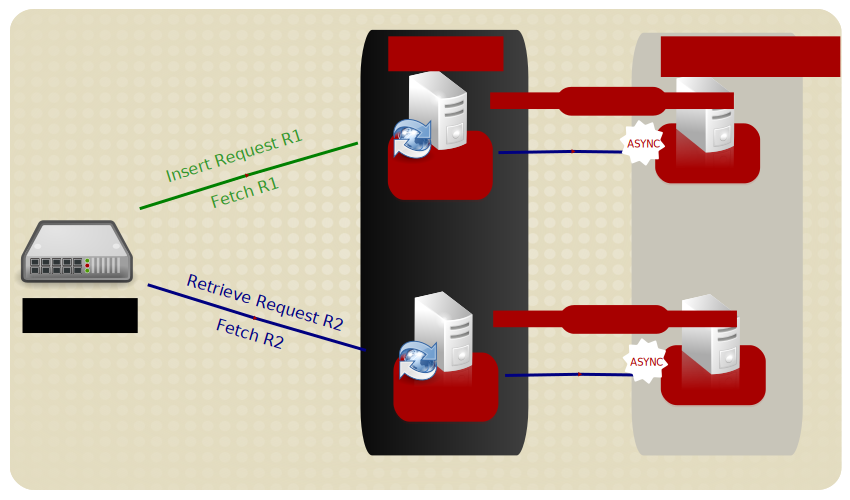
\includegraphics[scale=0.4]{../img/infinispan-example.png}
    \end{center}
  \end{frame}

  \begin{frame}{Base de données spécialisées}
    \begin{block}{Qu'est ce qu'une base de données spécialisés ?}
      \begin{itemize}
        \item orienté ou optimisé pour un certain modèle de données
        \item produit indépendant ou construit sur une base de données "généraliste"
        \begin{itemize}
         \item PostGIS - extension géospatial pour Postgresql
        \end{itemize}
      \end{itemize}
    \end{block}
    \begin{center}
      \includegraphics[scale=0.4]{../img/PostGIS-database.png}
    \end{center}
  \end{frame}

  \begin{frame}{ETL, un exemple d'outil}
    \begin{block}{Propos et intérêt des ETLs}
      \begin{itemize}
        \item migrer les données d'une base de données à une autre
        \item TODO
      \end{itemize}
    \end{block}
  \end{frame}
}

\ifslide {
  \mysubsection{Programmation distribuée}

\ifslide{
  \begin{frame}{Une longue et vielle histoire...}
   \begin{block}{Historique}
     \begin{itemize}
       \item DCE
       \item CORBA
       \item Java-RMI
       \item COM/DCOM
       \item EJB
       \item ...
     \end{itemize}
   \end{block}
  \end{frame}

  \begin{frame}{Enjeu}
   \begin{block}{Motivation}
     \begin{itemize}
       \item séparer le code entre différente instance physique
       \item tenu de charge, routage, balance de charge
       \item sécurité
     \end{itemize}
   \end{block}
  \end{frame}

  \begin{frame}{Remote Procedure Call}
    \begin{block}{Qu'est ce que RPC ?}
      \begin{itemize}
        \item base de nombreuses technologies (DCE, DCOM/COM,...)
        \item idée ancienne (1976)
        \item \mylink{http://tools.ietf.org/html/rfc707}{RFC 707}
      \end{itemize}
    \end{block}

    \begin{block}{Avantages/Inconvénients}
      \begin{itemize}
        \item Indépendance du transport
        \item Transformation des données
        \item Bloque le Client lors d’un appel à une procédure
        \item Echec possible en cas de problèmes réseaux
        \item Gestion difficile de reprise d’erreur
      \end{itemize}
    \end{block}
  \end{frame}

  \begin{frame}{MOM vs RPC}
    \begin{center}
      \includegraphics[scale=0.22]{img/mom-rpc.png}
    \end{center}
  \end{frame}

  \begin{frame}{Middleware orientés objets}
   \begin{block}{Motivation}
     \begin{itemize}
       \item invoqué des objets à distances (plutôt que récupérer des données)
       \item ex: DCE, DCOM, RMI, SOAP,...
     \end{itemize}
    \end{block}
  \end{frame}

  \begin{frame}{Ex: Java RMI}
    \begin{block}{Remote Method Invocation}
     \begin{itemize}
       \item originellement interopérable que entre machines virtuelles
       \item protocole sous jacent Java Remote Method Protocole (JRMP)
       \item étendu pour supporter CORBA (interopérabilité hors Java) : RMI-IIOP
     \end{itemize}
    \end{block}

    \begin{center}
      \includegraphics[scale=0.6]{img/rmi-stubs-skeletons.jpg}
    \end{center}
  \end{frame}

}

  \begin{frame}{Les Outils d'un projet informatique (2) }
    \begin{center}
      Le gestionnaire de source
    \end{center}
  \end{frame}
  \mysubsection{Transaction distribuée}

\ifslide{
  \begin{frame}
    \begin{block}{Transaction distribué}
      \begin{itemize}
        \item implique plusieurs ressources (transactionnelle)
        \item nécessite un \textbf{context}
        \begin{itemize}
          \item transparent pour l'application
          \item mais peut être explicite
        \end{itemize}
      \end{itemize}
    \end{block}
  \end{frame}

  \begin{frame}
    \begin{block}{Implémentation de la propagation}
      \begin{itemize}
        \item \textbf{context} doit être propagé
        \item utilise "ce qui existe"
        \begin{itemize}
          \item CORBA
          \item IIOP
          \item SOAP
          \item ...
        \end{itemize}
      \end{itemize}
    \end{block}

    \begin{block}{Impact sur le système transactionnel}
      \begin{itemize}
        \item implémentation définie limites et capacité
      \end{itemize}
    \end{block}
  \end{frame}

  \begin{frame}
    \begin{block}{\textit{Distributed Transaction Processing} (DTP)}
      \begin{itemize}
        \item défini par l'\textit{Open Group}
        \item implémenter (par exemple) en Java, par JTA
        \item défini l'API (XA) entre
        \begin{itemize}
          \item \textit{Ressource Manager} [RM] (ex: base de données SQL)
          \item \textit{Transaction Manager} [TM] (Transaction Manager)
        \end{itemize}
      \end{itemize}
    \end{block}
  \end{frame}


}

}
\mysubsection{Architecture orientée service (SOA)}

\ifbook{
  \paragraph{} L'\textbf{Architecture Orientée Services} - ou, en anglais \textit{Service Oriented
  Architecture (SOA)} est probablement l'un des termes les plus à la mode depuis le début des années
  2000. Fruits des années de réflexions sur l'\mylink{}{urbanisation} des systèmes d'informations,
  cette architecture de médiation propose une architecture pour concevoir des systèmes d'information
  très fortement découplé.

  \paragraph{} En effet, l'un des objectifs clairement avoué de cette architecture est de permettre
  la construction de systèmes d'information à l'aide de service hétérogènes, fonctionant sur des
  systèmes et des technologies complètement différentes. On cherche donc ainsi à réaliser des
  logiciels indépendants, exposants différents services métiers ou techniques, chacun
  \textbf{atomique}. Pour réaliser les différents traitements nécessaires à ses utilisateurs, une
  application effectue donc une série d'appel à différents services, et agrège les résultats, avant
  de les présenter à son utilisateur.

  \paragraph{} Néanmoins pour assurer le \textbf{fort découplage} promût par l'architecture, il est
  important qu'une application ne devienne pas adhérante à un service, ce qui reste possible, même
  si ce dernier s'exécute sur une autre machine, dans une autre technologie. L'architecture prévoit
  donc aussi la mise en place de \textbf{contrat de service}, jouant là un rôle similaire à celui
  des \textbf{interfaces} dans le langage de programmation Java. Ces contrats sont placés dans un
  \textbf{annuaire} de service, permettant aux logiciels clients d'accéder de manière transparente
  aux services capables d'assurer les fonctionnalités souhaitées.

  \paragraph{} L'architecture orientée services reste néanmoins très abstraite et n'impose aucune
  technologie pour réaliser les différents éléments nécessaire à son implémentation. Notament, SOA
  ne définit que de manière très lâche les mécanimes à mettre en place pour effectuer la
  communication avec le service, laissant la place à plusieurs protocoles possibles pour
  l'implémenter.

  \mysubsubsection{WebServices}

  \paragraph{} Depuis les débuts de l'informatique, de nombres technologies, standards et
  protocoles\footnote{On ne citera ici que quelques exemples, parmi les plus célèbres: RPC, CORBA,
  COM/DCOM, RPC ...} ont été définies pour permettre de aisément répartir la réalisation de traitements
  entre plusieurs machines distinctes. Nous avons déjà vu par exemple le standard EJB. Au fur et à
  mesure que les systèmes d'information se sont urbanisés, les problématiques d'interopérabilités de
  ces technologies sont apparus de plus en plus clairement, surtout en comparaison avec les progrès
  manifestes réalisés dans le domaine par les technologies internet.

  \paragraph{} S'inspirant donc des idées fortes de ces dernières\footnote{On pense surtout ici au
  côté ouvert du protocole HTTP et de sa communication en format texte (HTML)}, les
  \textit{WebServices} sont donc apparus à leur tour. Utilisant les standards issues de l'émergence
  d'internet - XML, XSD, et définissant son propre ensemble de spécification, dont un format
  d'échange XML nommée \textbf{SOAP}, les \textit{WebServices} ont donc mis tout les chances de
  leurs côtés pour assurer leur interopérabilité.

  \paragraph{} Néanmoins, la complexité des \textit{WebServices} et le foisonement de spécifications
  autour d'elles - ajouté au fait que, malgré les précautions prises, l'interopérabilité fût souvent
  difficile à obtenir, spécialement lorsque les structures de données échangés devinrent de plus en
  plus élaborées, posant encore de des réelles difficultés. Les outils qui devaient résoudre ces
  difficultés ne virent que rarement le jour, et ne tenèrent que rarement leurs promesses.

  \begin{center}
    \includegraphics[scale=0.8]{img/ws-star.png}
  \end{center}

  \paragraph{} Un autre aspect, très puissant, des \textit{WebServices} estt la capacité, pour un
  service consommateur de \textbf{négocier} son niveau de protocole. Ceci permettant de gérer les
  problématiques de montée de version d'un service, sans impacter les applications clientes, puisque
  celles-ci devaient être en mesure d'indiquer quel niveau de service - la version du service en
  langage vernaculaire, elle est en mesure d'utiliser.

  \paragraph{} Pour assurer cet aspect et renforcer le découplage entre les consommateurs de
  services et les producteurs, les spécifications \textit{WebServices} prévoient aussi l'utilisation
  d'un annuaire de service, accompagné de sa propre sémantique et norme: UDDI (\textit{Universal
  Description and Discovery Integration}). Ce dernier, dont l'API n'est pas malheureusement la plus
  transparente, a comme fonction de transmettre le point d'accès - ou \textit{endpoint} en anglais,
  soit l'URL a invoquer pour utiliser le service, selon le \textbf{contrat} de service demandé.

  \paragraph{} L'engouement pour les \textit{WebServices} ont rapidement amené à étendre leur
  utilisation. On n'a donc défini des APIs pour standardiser l'utilisation de ces derniers comme
  protocole de communication pour un MOM ou même en tant que canal de communication pour un échange
  RPC ! La nature très verbeuse du protocole ayant souvent un prix en termes de performance, des
  implémentations remplaçant l'utilisation de HTTP et XML par un protocole binaire\footnote{Tel que
  le project Java Hessian} ont vu le jour - même si cette approche peut sembler contre nature...

  \paragraph{} Aujourd'hui, les \textit{WebServices} disposent donc d'un écosystème riche et fourni,
  mais l'enthousiasme les concernants à largement réduit, suite aux difficultés rencontrées sur le
  terrain, lors de leurs implémentations. Si ils se révèlent une technologie robuste et
  intéropérable pour mettre en place des services métiers complexes - et souvent orientés "écriture
  de données", ils se sont souvent révélés inadapté à des cas d'utilisation plus simple, et aussi
  souvent orienté "lecture" de données.

  \paragraph{} Le fait que Google a retiré depuis maintenant plusieurs années son API SOAP
  \footnote{au profit d'un nouveau type d'API que nous allons maintenant évoquée} est un indicateur
  fort du recul des \textit{WebServices} comme solution "parfaite" pour la conception de services
  distants ou internet.

  \paragraph{} \paragraph{} \textit{Remarque: Si la notion d'architecture orienté service n'impose
  en aucun cas l'utilisation de WebService\footnote{Pour s'en convaincre, il suffira d'étudier la
  page Wikipedia associée à
  \mylink{http://en.wikipedia.org/wiki/Service_Oriented_Architecture_Fundamentals}{SOA}}, ces
  derniers adressent la plupart des contraintes et recommandations de SOA. Il faut néanmoins noter
  que des projets respectant les principes de SOA ont  été implémenté, avec succès, à l'aide
  d'autres technologie telle RMI ou ReST. Il est donc important de retenir que SOA n'implique pas
  obligatoirement l'utilisation de \textit{WebServices}}.
}


\ifslide{
  \begin{frame}{Web Service}
    \begin{block}{Qu'est qu'un \textit{Web Service}}
      \begin{itemize}
        \item même concept que le Web mais appliqué la communication entre machine
        \item donc moins orienté "lecture" (plus d'opération d'écriture)
        \item plus "dynamic"
        \item support des environements hétérogènes
      \end{itemize}
    \end{block}
  \end{frame}

  \begin{frame}{Web Service}
    \begin{block}{Indépendance du \textit{End Point}}
      \begin{itemize}
        \item traitement réparti
        \item maintenance du noeud indépendante
        \item négociation de protocole
        \item couplage lâche
      \end{itemize}
    \end{block}
  \end{frame}

  \begin{frame}{Web Service}
    \begin{block}{Composition de protocole}
      \begin{itemize}
        \item architecture modulaire
        \item complexité géré par les outils
        \item extensibilité apporté par XML
      \end{itemize}
    \end{block}

    \begin{center}
      \includegraphics[scale=0.8]{img/web-services.png}
    \end{center}

  \end{frame}

  \begin{frame}{Web Service}
    \begin{center}
      \includegraphics[scale=0.8]{img/ws-star.png}
    \end{center}
  \end{frame}

  \begin{frame}
    \begin{block}{MOM et RPC... en WS !}
      \begin{itemize}
        \item XML-RPC
        \item publish/subscribe
        \item pièce jointe
      \end{itemize}
    \end{block}

    \begin{block}{Indépendance du transport}
      \begin{itemize}
        \item HTTP
        \item TCP
        \item Binaire !
      \end{itemize}
    \end{block}
  \end{frame}

  \begin{frame}
    \begin{block}{Mais aussi...}
      \begin{itemize}
        \item transaction
        \item sécurité
        \item ...
      \end{itemize}
    \end{block}

    \begin{block}{Découverte de Service et Annuaire}
      \begin{itemize}
        \item UDDI
        \item WS-Discovery
      \end{itemize}
    \end{block}
  \end{frame}
}

\ifbook{
  \mysubsubsection{ReST - le successeur des WebServices ?}

  \paragraph{} Si les \textit{WebServices} sont clairement issus du monde de l'industrie et le fruit
  d'un travail de standardisation, ReST n'est pas un standard, ni même une technologie réellement
  définie. ReST - ou \textit{Representationnal State Transfer} en anglais, est en quelque sorte le
  fruit d'un analyse des bonnes pratiques, en terme d'architecture, qui ont émergés sur l'ensemble
  de l'internet.

  \paragraph{} Sans rentrer dans les détails de sa théorie\footnote{On pourra là aussi consulter la
  page wikipédia consacré à \mylink{TODO}{ReST}.}, nous pourrons retenir que ReST tant à simplifier
  la communication entre le client et le serveur en exploitant autant que possible les mécanismes
  offerts par le protocole HTTP (utilisation de l'ensemble des opérations du protocole, soit PUT et
  DELETE, et non seulement des méthodes POST, mais aussi utilisation d'une sémantique très
  expressives dans les URLs des services), plutôt que de transmettre de descripteurs multiples en
  XML, par exemple.

  \paragraph{} Sur le format de données, ReST n'impose rien, mais, de plus en plus, l'usage impose
  l'utilisation du format JSON, issu du monde Javascript, et considéré par une partie de
  l'industrie, comme beaucoup plus clair et approprié que XML. Néanmoins, si les services de types ReST
  ont d'indéniables avantages, il est peut être un peu hasardeux de les positionner comme une
  technologie de remplacement des \textit{WebServices}.

  \paragraph{} En effet, si il est appararu clairement que ces derniers n'étaient pas adapté à la
  mise en place de service de consultation donnée à grande échelle (sur internet), les services de
  types ReST posent de grandes difficultés dans la réalisation de services applicatifs - ces
  derniers ne proposent que peu de solutions pratiques ou standard dans le domaine de la sécurité,
  ou de la transaction, par exemple.

  \paragraph{} En guise de conclusion de très haut niveau, on pourra donc retenir que les services
  de types ReST sont généralement très adaptés à la mise en place de services en "lecture", devant
  fournir un accès des données pour de buts de consultations. À l'inverse, les \textit{WebServices}
  se révèlent un ensemble de standards assez complet pour la conception de services nécessitant
  la modification ou l'ajout de données.\footnote{Il s'agit bien évidemment d'une conclusion très
  générale, pour éclairer le lecteur sur ces technologies, et non de la définition d'une règle
  absolu et unilatéral. Face au choix Rest ou \textit{WebServices}, le lecteur devra prendre soin
  d'analyser en détail les cas d'utilisations et le contexte techniques avant d'opter pour l'une ou
  l'autre des technologies.}
}


\ifbook{
  \mysubsubsection{SOA et Bus logiciel (ESB)}

  \paragraph{} Faisons un rapide bilans des nombreuses technologies évoqués dans ce chapitre et les
  précédents de cette ouvrage. On se rend compte ainsi que le système d'informations, désormais très
  urbanisé, contient beaucoup d'élément hétérogènes:

  \begin{itemize}
    \item \textit{WebServices} et service ReST,
    \item MOM,
    \item BPM et leur moteur de règles,
    \item ...
  \end{itemize}

  \paragraph{} Il apparait évident qu'une application métier pour réaliser ses fonctionnalités va
  devoir faire appel à ses différents éléments et que très rapidement un besoin
  d'\textbf{orchestration} de ces différents services va apparaitre. En effet, dans une vision
  \textbf{opérationnel} du système d'information, il apparait important, si ce n'est essentiel, de
  disposer, entre les consommateurs de services et leurs fournisseurs d'un mécanisme pour effectuer
  de la \textbf{répartition de charge} ou du simple \textbf{routage}, comme par exemple lors de
  l'interromption, pour maintenance ou mise à une jour, d'une instance d'un service.

  \paragraph{} C'est de ce besoin qu'a émergé la notion de \textit{Entreprise Service Bus (ESB)}. En
  effectuant un parallèle avec les bus de communication électroniques, ces solutions se positionnent
  donc comme un intermédiaire similaire, et pourtant presque invisible, entre les consommateurs et
  fournisseurs de services.

  \paragraph{} En outre, ces outils permettent aussi d'effectuer des \textbf{transformation} de
  données ou de protocole, pour permettre à deux services - à priori incompatibles, de communiquer
  malgré tout. À ce regard, les ESB sont les hérities des EAI - \textit{Entreprise Application
  Integration}, qui effectue le même genre de synthèse, mais sur des technologies et protocoles
  non standard issus des logiciels propriétaires.\footnote{Là encore, le lecteur prendra soin de
  noter que cette synthèse est relativement grossière et quelques peu simpliste.}

  \begin{center}
    \includegraphics[scale=1]{img/esb.png}
  \end{center}

  \paragraph{} \textit{\mylink{http://en.wikipedia.org/wiki/BPEL}{BPEL}: Business Process Execution
  Language est un langage de programmation destiné à l'exécution des procédures d'entreprise.}
}

\ifslide{

  \begin{frame}
    \begin{block}{SOA}
      \begin{itemize}
        \item architecure
        \item \textit{loose coupling}
        \item fonctionnement par contrat
      \end{itemize}
    \end{block}

    \begin{block}{ESB}
      \begin{itemize}
        \item orchestration
        \item analogue à un Bus électronique
      \end{itemize}
    \end{block}
  \end{frame}

  \begin{frame}{ESB}
    \begin{center}
      \includegraphics[scale=1]{img/esb.png}
    \end{center}
  \end{frame}

  \mysubsection{ETL, EAI et autres middlewares}
    %TODO: not cover in the book
}



\ifslide {
  \begin{frame}{Les Outils d'un projet informatique (3) }
    \begin{center}
      Outil de gestion de tâche (\textit{bugtracking}
    \end{center}
  \end{frame}

  \mysection{D - Mise à échelle et production (12/01/2012)}

\abstractframe{Cette partie évoque les problématiques liées à la mise en production
et la surveillance d'une application et des \textit{middlewares} qu'elle
utilise.}{../img/overview-monitoring.png}

\mysubsection{Problématique de performances des middlewares}

\ifslide{
  \begin{frame}
    \begin{block}{Performance et mise production des \textit{middlewares}}
      \begin{itemize}
        \item au coeur du problème
        \item complexité
        \item charge élévée
        \item attente accrue
        \item plus de période de repos
      \end{itemize}
    \end{block}

    \begin{block}{Effet "boite noire"}
      \begin{itemize}
        \item l'application en elle même
        \item rôle et fonctionnement des \textit{middleware}
        \item complexité et distribution
      \end{itemize}
    \end{block}
  \end{frame}
}


\mysubsection{Stratégie de mise à l'échelle (Ferme, clustering...)}

\ifslide{
  \begin{frame}
    \begin{block}{Objectifs}
      \begin{itemize}
        \item Tolérance aux pannes (et reprise sur pannes)
        \item Haute Disponibiités
      \end{itemize}
    \end{block}
    \begin{block}{Techniques}
      \begin{itemize}
        \item Balance de charge
        \item Ferme de serveurs
        \item \textit{Cluster}
      \end{itemize}
    \end{block}
  \end{frame}
}

\mysubsection{Indicateur, surveillance et alertes}

\ifslide{
  \begin{frame}
    \begin{block}{Problématique de la surveillance}
      \begin{itemize}
        \item Que faut il surveiller ? Que faut il mesurer ?
        \item Quelles alertes ?
      \end{itemize}
    \end{block}
  \end{frame}

  \begin{frame}
    \begin{center}
    \Large{Le \textit{monitoring} applicatif est forcément spécifique !}
    \end{center}

    \begin{block}{Définir sa stratégie}
      \begin{itemize}
        \item Maitriser la complexité de ses applicatifs
        \item Choisir ses indicateurs
        \item Donner les moyens de surveiller son applicatifs
      \end{itemize}
    \end{block}
  \end{frame}

  \begin{frame}{\textit{Time to draw some clever shit on the board...}}
  \end{frame}

}


  \begin{frame}
    \begin{block}{\textit{This is the End...}}
      \begin{itemize}
        \item Questions sur le cours ? Remarques ?
        \begin{itemize}
          \item \mylink{mailto:belaran@gmail.com}{belaran@gmail.com} (perso)
        \end{itemize}
        \item Besoin d'aide ?
        \begin{itemize}
          \item \mylink{mailto:belaran@gredhat.com}{belaran@redhat.com} (pro)
          \item \mylink{mailto:romain@gredhat.com}{romain@redhat.com} (pro)
        \end{itemize}
      \end{itemize}
    \end{block}
  \end{frame}
}
